\subsection{M.PC.SV - Schedule Variance e M.PC.CV - Cost Variance}

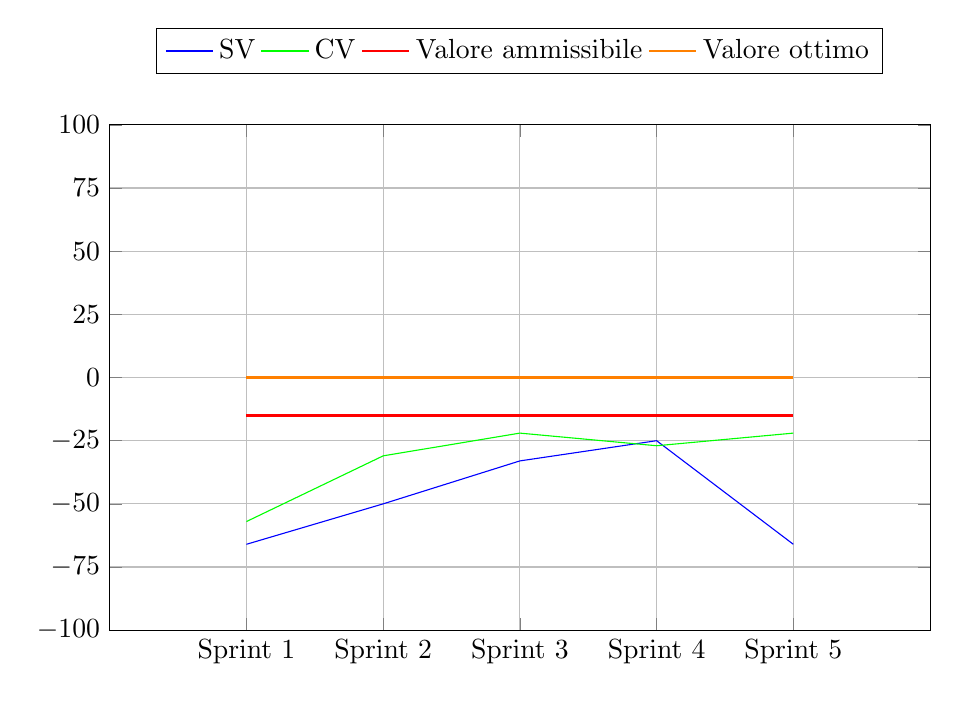
\begin{tikzpicture}
    \begin{axis}[
        width=12cm, height=8cm,
        ymin=-100, ymax=100,
        xmin=0, xmax=6,
        ytick distance=25,
        xtick={1, 2, 3, 4, 5},
        xticklabels={Sprint 1, Sprint 2, Sprint 3, Sprint 4, Sprint 5},
        xlabel={},
        ylabel={},
        grid=major,
        scaled ticks=false,
        legend style={at={(0.5,1.1)}, anchor=south, legend columns=-1},
    ]
    \addplot[color=blue] coordinates {(1, -66) (2, -50) (3, -33) (4, -25) (5, -66)};
    \addlegendentry{SV}
    \addplot[color=green] coordinates {(1, -57) (2, -31) (3, -22) (4, -27) (5, -22)};
    \addlegendentry{CV}
    \addplot[red, thick] coordinates {(1, -15) (5, -15)};
    \addlegendentry{Valore ammissibile}
    \addplot[orange, thick] coordinates {(1, 0) (5, 0)};
    \addlegendentry{Valore ottimo}
    \end{axis}
\end{tikzpicture}
\subsubsection{RTB}
La Schedule Variance presenta valori negativi con un valore assoluto notevolmente superiore al valore ammissibile, questo è dovuto a una pianificazione
ottimistica ed errata del lavoro da svolgere, come visto nel grafico precedente l'Earned Value a ogni sprint è stato notevolmente più basso rispetto al Planned Value
e questo ha portato ad avere valori della Scheule Variance bassi e che non rispettano il valore ammissibile voluto.
Con il passare del tempo è andata ad aumentare indicando inizialmente un miglioramento, con lo sprint 5 è stata effettuata una pianificazione di tutte le attività
necessarie alla realizzazione del Proof of Concept, queste non sono state successivamente completate causando un eccessivo abbassamento del valore della metrica.
La Cost Variance presenta valori negativi inferiori rispetto al valore ammissibile perché, durante gli sprint, sono state impiegate ore di lavoro per attività non completate. 
Questo ha provocato un aumento dell'Actual Cost senza un corrispondente incremento dell'Earned Value.
Successivamente, si osserva un miglioramento della metrica. Questo accade perché il costo delle ore impiegate per attività non completate grava sullo sprint in cui erano pianificate, 
senza generare un aumento dell'EV. Tuttavia, quando queste attività vengono completate in sprint successivi entro il tempo previsto, la CV migliora.
Ciò avviene perché nel momento in cui attività iniziate durante sprint precedenti vengono completate l'Earned Value aumenta notevolmente mentre l'incremento dell'Actual Cost è limitato al solo completamento delle attività.